%&bericht



\documentclass[
   ngerman          % neue deutsche Rechtschreibung
  ,a4paper          % Papiergrösse
% ,twoside          % Zweiseitiger Druck (rechts/links)
% ,10pt             % Schriftgrösse
% ,11pt
  ,12pt
  ,pdftex
%  ,disable         % Todo-Markierungen auschalten
]{report}

% Bitte die Codierung Ihrer Dateien auswählen:
% \usepackage[latin1]{inputenc}    % Für UNIX mit ISO-LATIN-codierten Dateien
% \usepackage[applemac]{inputenc}  % Für Apple Mac
% \usepackage[ansinew]{inputenc}   % Für Microsoft Windows
\usepackage[utf8]{inputenc}        % UTF-8 codierte Dateien
                                   % Dieses Dokument ist unter Unix erstellt, daher
                                   % wird diese Input-Codierung benutzt.

\usepackage{bericht}
%\usepackage[onehalfspace]{setspace}
\usepackage{graphicx}
\usepackage{color}
\usepackage{transparent}
\graphicspath{Bilder/}

%\usepackage[backend=biber]{biblatex}

\usepackage[]{biblatex}

\addbibresource{Literaturverzeichnis2.bib}
%\usepackage[backend=bibtex,style=numeric]{biblatex}
%\bibliographystyle{unsrt}
%\citep[vgl.][]{modOpSys}
%\addcontentsline{toc}{section}{Literatur}



%% ACHTUNG, wenn man eine eigene Formatdatei (bericht.fmt) benutzt, werden Änderungen an bericht.sty
%% erst wirksam, wenn die Format-Datei neu erzeugt wurde!!!
%% Genauer alle Änderungen, die textuell vor der nächsten Zeile ".... endofdump...." stehen
%% werden erst wirksam, wenn die Formatdatei neu erzeugt wurde
\csname endofdump\endcsname

%%%%%%%%%%%%%%%%%%%%%%%%%%%%%%%%%%%%%%%%%%%%%%%%%%%%%%%%%%%%%%%%%%%%%%%%%%%%%%%
%% Angaben zur Arbeit
%%%%%%%%%%%%%%%%%%%%%%%%%%%%%%%%%%%%%%%%%%%%%%%%%%%%%%%%%%%%%%%%%%%%%%%%%%%%%%%

\newcommand{\Autor}{Lorenz Scherrer}
\newcommand{\MatrikelNummer}{4711}
\newcommand{\Kursbezeichnung}{ka-tinf21b3}

\newcommand{\FirmenName}{SICK}
\newcommand{\FirmenStadt}{Waldkirch}
\newcommand{\FirmenLogoDeckblatt}{\fbox{
\includegraphics[width=3cm]{Bilder/lion.png}}}

% Falls es kein Firmenlogo gibt:
%  \newcommand{\FirmenLogoDeckblatt}{}

\newcommand{\BetreuerFirma}{Titel Vorname Nachname}
\newcommand{\BetreuerDHBW}{Titel Vorname Nachname}

%%%%%%%%%%%%%%%%%%%%%%%%%%%%%%%%%%%%%%%%%%%%%%%%%%%%%%%%%%%%%%%%%%%%%%%%%%%%%%%%%%%%%

% Wird auf dem Deckblatt und in der Erklärung benutzt:
\newcommand{\Was}{Projektarbeit}
%\newcommand{\Was}{Projektrarbeit}
%\newcommand{\Was}{Studienarbeit}
%\newcommand{\Was}{Bachleorarbeit}

%%%%%%%%%%%%%%%%%%%%%%%%%%%%%%%%%%%%%%%%%%%%%%%%%%%%%%%%%%%%%%%%%%%%%%%%%%%%%%%%%%%%%

\newcommand{\Titel}{Fortentwichlung und Neugestaltung der Software des LMS4000 Demokoffers}
\newcommand{\AbgabeDatum}{1. Oktober 2022}

\newcommand{\Dauer}{12 Wochen}

% \newcommand{\Abschluss}{Bachelor of Engineering}
\newcommand{\Abschluss}{Bachelor of Science}

\newcommand{\Studiengang}{Informatik / Informationstechnik}
% \newcommand{\Studiengang}{Informatik / Angewandte Informatik}

\hypersetup{%%
  pdfauthor={\Autor},
  pdftitle={\Titel},
  pdfsubject={\Was}
}

%%%%%%%%%%%%%%%%%%%%%%%%%%%%%%%%%%%%%%%%%%%%%%%%%%%%%%%%%%%%%%%%%%%%%%%%%%%%%%%

% Wenn \includeonly{..} benutzt wird, werden nur diese Kaptitel ausgegeben.
\includeonly{
  abk
 ,einleitung
 ,grundlagen
 ,umsetzung
 ,fazit
 ,changelog
}

%%%%%%%%%%%%%%%%%%%%%%%%%%%%%%%%%%%%%%%%%%%%%%%%%%%%%%%%%%%%%%%%%%%%%%%%%%%%%%%

% Benutzt man das "biblatex"-Paket, dann muß das hier stehen:
% siehe auch die mit BIBLATEX markierten Zeilen in bericht.sty
%\bibliography{bericht}



\begin{document}

%%%%%%%%%%%%%%%%%%%%%%%%%%%%%%%%%%%%%%%%%%%%%%%%%%%%%%%%%%%%%%%%%%%%%%%%%%%%%%%

\begin{titlepage}
\begin{center}
\vspace*{-2cm}
\FirmenLogoDeckblatt\hfill
\includegraphics[width=4cm]{Bilder/dhbw-logo.png}\\[2cm]
%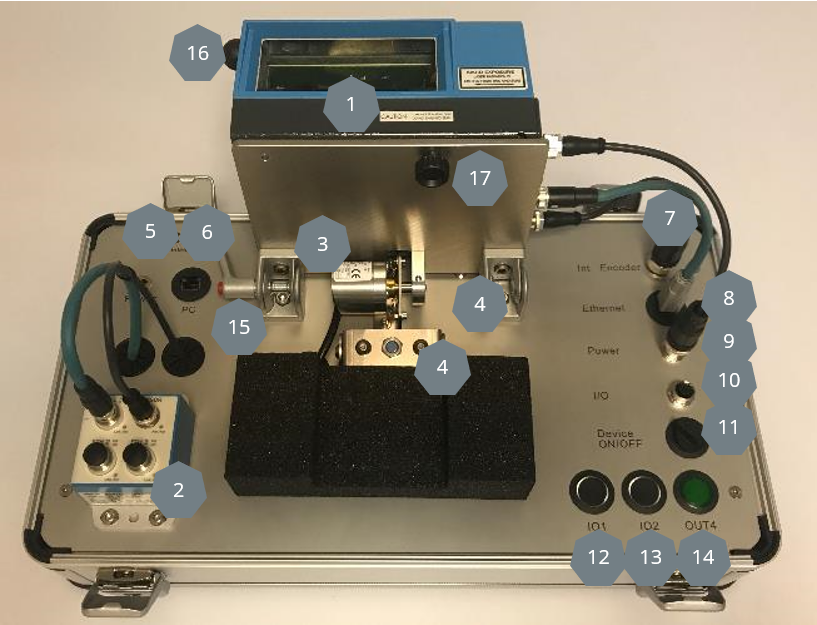
\includegraphics[width=13cm]{Bilder/Demokoffer.png}
{\Huge \Titel}\\[1cm]
{\Huge\scshape \Was}\\[1cm]
{\large für die Prüfung zum}\\[0.5cm]
{\Large \Abschluss}\\[0.5cm]
{\large des Studienganges \Studiengang}\\[0.5cm]
{\large an der}\\[0.5cm]
{\large Dualen Hochschule Baden-Württemberg Karlsruhe}\\[0.5cm]
{\large von}\\[0.5cm]
{\large\bfseries \Autor}\\[1cm]
{\large Abgabedatum \AbgabeDatum}
\vfill
\end{center}
\begin{tabular}{l@{\hspace{2cm}}l}
Bearbeitungszeitraum	         & \Dauer 			\\
Matrikelnummer	                 & \MatrikelNummer		\\
Kurs			         & \Kursbezeichnung		\\
Ausbildungsfirma	         & \FirmenName			\\
			         & \FirmenStadt			\\
Betreuer der Ausbildungsfirma	 & \BetreuerFirma		\\
Gutachter der Studienakademie	 & \BetreuerDHBW		\\
\end{tabular}
\end{titlepage}

%%%%%%%%%%%%%%%%%%%%%%%%%%%%%%%%%%%%%%%%%%%%%%%%%%%%%%%%%%%%%%%%%%%%%%%%%%%%%%%


%%%%%%%%%%%%%%%%%%%%%%%%%%%%%%%%%%%%%%%%%%%%%%%%%%%%%%%%%%%%%%%%%%%%%%%%%%%%%%%
%% Descr:       Vorlage für Berichte der DHBW-Karlsruhe, Erklärung
%% Author:      Prof. Dr. Jürgen Vollmer, vollmer@dhbw-karlsruhe.de
%% $Id: erklaerung.tex,v 1.11 2020/03/13 14:24:42 vollmer Exp $
%% -*- coding: utf-8 -*-
%%%%%%%%%%%%%%%%%%%%%%%%%%%%%%%%%%%%%%%%%%%%%%%%%%%%%%%%%%%%%%%%%%%%%%%%%%%%%%%

% In Bachelorarbeiten muss eine schriftliche Erklärung abgegeben werden.
% Hierin bestätigen die Studierenden, dass die Bachelorarbeit, etc.
% selbständig verfasst und sämtliche Quellen und Hilfsmittel angegeben sind. Diese Erklärung
% bildet das zweite Blatt der Arbeit. Der Text dieser Erklärung muss auf einer separaten Seite
% wie unten angegeben lauten.

\newpage
\thispagestyle{empty}
\begin{framed}
\begin{center}
\Large\bfseries Erklärung
\end{center}
\medskip
\noindent
% siehe §5(3) der \enquote{Studien- und Prüfungsordnung DHBW Technik} vom 29.\,9.\,2017 und Anhang 1.1.13
Ich versichere hiermit, dass ich meine \Was mit dem Thema:
\enquote{\Titel}
selbstständig verfasst und keine anderen als die angegebenen Quellen und Hilfsmittel benutzt habe. Ich versichere zudem, dass die eingereichte elektronische Fassung mit der gedruckten Fassung übereinstimmt.
\vspace{3cm}
\noindent
\underline{\hspace{4cm}}\hfill\underline{\hspace{6cm}}\\
Ort~~~~~Datum\hfill Unterschrift\hspace{4cm}
\end{framed}

%\vfill
%\emph{Sofern  vom Dualen Partner ein Sperrvermerk gewünscht wird, ist folgende Formulierung
%zu verwenden:}
%\begin{framed}
%\begin{center}
%\Large\bfseries Sperrvermerk
%\end{center}
%\medskip
%\noindent
%Der Inhalt dieser Arbeit darf weder als Ganzes noch in Auszügen Personen
%außerhalb des Prüfungsprozesses und des Evaluationsverfahrens zugänglich gemacht
%werden, sofern keine anderslautende Genehmigung vom Dualen Partner vorliegt.
%\end{framed}

%%%%%%%%%%%%%%%%%%%%%%%%%%%%%%%%%%%%%%%%%%%%%%%%%%%%%%%%%%%%%%%%%%%%%%%%%%%%%%%
\endinput
%%%%%%%%%%%%%%%%%%%%%%%%%%%%%%%%%%%%%%%%%%%%%%%%%%%%%%%%%%%%%%%%%%%%%%%%%%%%%%%

%C:/Users/loren/DHBW_Karlsruhe/T1000/T1000/bericht.sty
%%%%%%%%%%%%%%%%%%%%%%%%%%%%%%%%%%%%%%%%%%%%%%%%%%%%%%%%%%%%%%%%%%%%%%%%%%%%%%%


\newpage
\tableofcontents           % Inhaltsverzeichnis hier ausgeben
\listoffigures             % Liste der Abbildungen
\listoftables              % Liste der Tabellen
\lstlistoflistings         % Liste der Listings
\listofequations           % Liste der Formeln

% Jetzt kommt der "eigentliche" Text
\include{abk}              % Abkürzungsverzeichnis


\chapter{Einleitung}
\doublespacing
\section{Vorwort}
Dieser Bericht handelt von den Tätigkeiten während der Praxisphase vom 18.10.2021
bis zum 10.01.2022 in der Abteilung Distance & Ranging BU83 bei der
SICK AG in Waldkirch. Ziel war die Fortentwichlung und Neugestaltung der Software des LMS4000 Demokoffers.



\section{Einleitung}
Der LMS4000 ist ein 2D-LiDAR(Light Detection and Ranging)-Sensor der es ermöglicht präzise Vermessungen schnell bewegender, kleiner und großer Objekte unabhängig von ihrer, Farbe oder Oberflächenbeschaffenheit.

Dieser LiDAR-Sensor wird mithilfe des Demokoffers für den Vertrieb demonstriert. Der Koffer beinhaltet mit dem LMS4000 noch drei weitere Sensoren. Zwei von diesen Sensoren sind Metallsensoren, sogenannte Inits, sie werden dazu verwendet, die genaue Winkelposition des LMS4000 zu bestimmen. Der letzte Sensor ist ein Encoder, dieser bestimmt die Veränderung der Position des LMS4000. Mit diesen drei Sensoren kann die Winkelposition des LMS4000 bestimmt werden. Eine SIM1000 wird dazu genutzt, die Daten, die die vier Sensoren liefern, zu erfassen, auszuwerten und zu archivieren (Beschreibung des Demokoffers erweitern).

Mit dem Programm AppStudio ist es möglich, eine App für die SIM1000 zu schreiben. Diese App weist jedem 2D-Scan des LMS4000 eine Winkelposition zu. Somit macht die App es möglich 3D-Bilder mit 60Hz von den möglichen 600Hz des LMS4000 aufzunehmen für 10 Sekunden. Die Bildrate schöpft das Potenzial des LMS4000 nicht aus.

(Um den LMS4000 besser im Vertrieb zu präsentieren wäre es günstig die Bildrate zu erhöhen). Um die Bildrate des Demokoffers zu erhöhen, sollen zwei Apps zusammen arbeiten. Der ScanDriver der von Chris Jorna und die Demokoffer App von Manuel Würzburger..\cite{Ansmann.op.1997,Basler.2016,Fujii.2005,Ierusalimschy.op.2016,Ierusalimschy.2006,Jung.2007,Kuhnel.2012,.,Martin.2013,Young.2014}

\newpage

\section{SICK AG}
\subsection{Geschichte}
Bereits 1946 wurde die heutige SICK AG von Erwin Sick in München gegründet. 1952 hatte
das Unternehmen dann seinen ersten wirtschaftlichen Durchbruch mit der Vorstellung eines
Unfallschutz-Lichtvorhangs auf der Internationalen Werkzeugmesse in Hannover. Der Erfolg
stellte sich ein und die SICK AG ist heute einer der führenden Herstellern und Entwickler
von Sensoren und Sensorlösungen für die Bereiche Fabrik-, Logistik- und Prozessautomation.
1956 zieht das damals 25 Mitarbeiter zählende Unternehmen von München an den heutigen
Standort Waldkirch. Im Jahre 1988 verstirbt Erwin Sick und seine Frau Gisela Sick führt das
Unternehmen als Hauptgesellschafterin fort. 1996 wird eine Umfirmierung des Unternehmens
von der Erwin Sick GmbH in eine Aktiengesellschaft durchgeführt. Der Hauptteil der Aktien
(95%) ist weiterhin in Familienbesitz. Die Restlichen 5% sind Mitarbeiteranteile. Somit ist das
Unternehmen nicht Börsen notiert und kann weiterhin nach Vorstellungen der Gründerfamilie
geführt werden mit nachhaltiger Wachstums Orientierung. Heute umfasst die SICK AG über 50
Tochtergesellschaften und Beteiligungen sowie zahlreiche Vertretungen rund um den Globus. Im
Geschäftsjahr 2021 erzielte das Unternehmen einen Umsatz von 1.964 Millionen Euro
und zählt Weltweit über 10.000 Mitarbeiter.

\begin{figure}[h]
\centering

\includegraphics[width=13cm]{Bilder/SICK AG Hauptsitz.jpg}
\caption{Hauptstandort der SICK AG in Waldkirch}
\label{SICK_AG_Hauptsitz}
\end{figure}


\subsection{Unternehmensstruktur}
Wie jedes größere Unternehmen ist auch die SICK AG in verschiedene Bereiche eingeteilt. 
Neben einigen Zentralbereichen, Corporate Departments (CDs) und Corporate Units (CUs), 
gibt es neun unterschiedliche Global Business Centers (GBCs). Jedes GBC hat eine weltweite 
Geschäftsverantwortung für einen bestimmten Technologiebereich. Hier liegt ebenso die 
Verantwortung für die Entwicklung, Produktion und das Produktmanagement von Produkten 
und Serviceleistungen.
Für jede Region gibt es eine zuständige Stelle, welche die Verantwortung für den Vertrieb und 
das Servicegeschäft übernimmt. Dieser Bereich ist in den Sales and Service Clusters (SSCs)
zusammengefasst.
Neben diesen Bereichen gibt es noch Global Intustry Centers (GICs), welche unter anderem 
die Verantwortung für das International Key Account Management (IKAM) und für Branchen 
in der Fabrik-, Logistik- und Prozessautomation innehaben. (SICK AG 2020d)
Die GBCs sind weiterhin in kleinere Einheiten, den sogenannten Business Units (BUs) 
aufgeteilt. Hier wird das Geschäftsfeld der GBC in verschiedene Produkt- und 
Dienstleistungskategorien unterteilt.
Je nach Größe und Ausrichtung einer BU, kann es vorkommen, dass eine weitere Unterteilung 
erfolgt. Hier wird Beispielsweise in Fachdisziplinen wie Entwicklung und Marketing 
aufgeschlüsselt.


\section{Ausgangssituation}

Die Hardware, mit der in diesem Projekt gearbeitet wird, ist der Demokoffer des LMS4000. Dieser wird im Vertrieb genutzt, um die Funktionen des LMS4000 zu demonstrieren. Auf dem Demokoffer lief bis vor kurzem die App von Silas Geschwender. Diese App nutzt nicht das volle Potenzial des LMS4000. Weshalb Manuel Würzburger mithilfe des ScanDrivers von Chris Jona das Potenzial des LMS4000 auszureisen. Der Ersteller hat an dieser neuen App weitergearbeitet, um sie fertig zustellen.

\begin{figure}[h!]
\centering
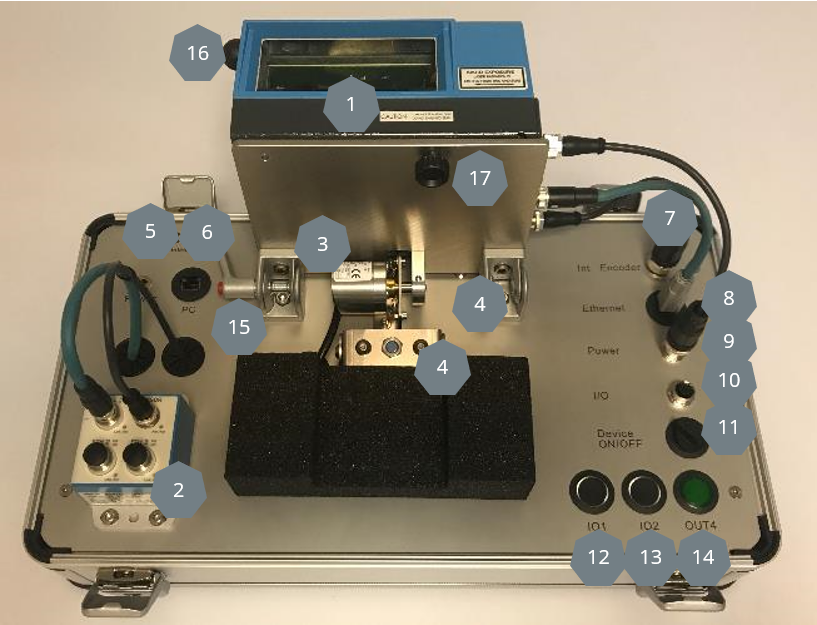
\includegraphics[width=13cm]{Bilder/Demokoffer.png}
\caption{Demokoffer}
\label{Demokoffer}
\end{figure}


\begin{table}[h!]

\begin{tabular}{ll}
1  & LM4111                                \\
2  & SIM1004                               \\
3  & Incremental Encoder                   \\
4  & Inductive Proximity Sensors           \\
5  & Power supply DC 24V                   \\
6  & Ethernet PC                           \\
7  & Internal Encoder                      \\
8  & Ethernet LMS4111                      \\
9  & Power supply LMS4111                  \\
10 & I/Os LMS4111                          \\
11 & Switch ON / OFF LMS4111               \\
12 & IO1 LMS4111                           \\
13 & IO2 LMS4111                           \\
14 & OUT4 LMS4111                          \\
15 & Locking lever for different positions \\
16 & Grab handle                          
\end{tabular}
\caption{Legende zur Abbildung 1.2}
\label{Legende zur Abbildung 12}
\end{table}

An dem Koffer sind vier Sensoren, zwei Metall Sensoren, die, die genau Gradzahl des LMS4000 bestimmen, einmal 0° und um die 90° Position zu bestimmen. Der Encoder kann Rotation feststellen und damit die Veränderung der Gradzahl.
Der LMS4000 nimmt ein 2D-Bild auf, welches einer Gradzahl zugewiesen wird. Die SIM1004 verarbeitet diese Daten zu einer Punktewolke.

\section{Aufgabenstellung}
Das Hauptziel ist es, die App auf eine stabile Version für den Vertrieb zu bringen. Fehler und Störungen sollen korrigiert werden. Ein weiteres Ziel ist es zu erforschen, welche die höchst mögliche Frequenzzahl ist, mit welcher aufgenommen werden kann. Die ursprüngliche App von Silas Geschwender konnte mit 60Hz für 10 Sekunden aufnehmen. Es muss bestimmt werden, mit welcher Herzfrequenz aufgenommen werden kann und die SIM noch stabil läuft. Auch soll das Design der App maßgeblich verändert werden. Die App besteht aus zwei Seiten, auf der ersten Seite stehen die Daten der Komponenten, Status des Demokoffers und hier können auch neue Scans aufgenommen werden. Der aktuelle Scann ist dort auch zu sehen, die älteren Scans sind auch der zweiten Seite zu sehen, wo sie auch heruntergeladen oder gespeichert werden können. Die Seite zum Aufnehmen der Scans und die Seite zum Einsehen der Scans sollen zusammengefasst werden.


\include{einleitung.tex}




\chapter{Grundlagen}

\section{Appstudio}
SICK AppSpace - Engineering-Framework für Ihre individuellen Sensoranwendungen

SICK AppSpace ist ein Ökosystem rund um programmierbare Sensoren und Geräte von SICK und individualisierte SensorApps. Als Teil einer dynamischen Entwickler-Community können Kunden eigenständig oder gemeinsam mit den Experten von SICK SensorApps erstellen. Mit diesen SensorApps lassen sich alle Anwendungen mit unterschiedlichsten Technologien lösen. Individualisierte SensorApps werden mit intelligenten Softwaretools und Algorithmen erstellt. Bestehende Lösungen für Track & Trace, Positionieraufgaben, Roboterführung oder Qualitätskontrolle können an die individuellen Bedürfnisse der Kunden angepasst werden; und völlig neue SensorApps können nach individuellen Anforderungen und absolut maßgeschneidert für bestehende Systeme erstellt werden. SICK AppSpace unterstützt heute eine Reihe von Geräten und Technologien, wie 2D-Vision, 3D-Vision, LiDAR, RFID oder Integrationsprodukte. Das SICK-AppSpace-Ökosystem besteht aus drei Hauptkomponenten. Zum einen aus der Hardware, das heißt programmierbare Sensoren, Sensorintegrationsmaschinen und andere Geräte. Zum anderen Software und Tools, das heißt die Werkzeuge zum Erstellen, Verteilen und Bereitstellen von SensorApps. Und als letzten Hauptkomponenten die Community, das heißt die Mitglieder des SICK AppSpace-Entwicklerclubs, die sich im SICK Support Portal und Konferenzen austauschen.

Die programmierbaren Geräte im SICK-AppSpace-Ökosystem bieten Raum für die Integration der kundenspezifischen SensorApps und ermöglichen so maßgeschneiderte Applikationslösungen. So werden je nach Anwendung völlig neue Lösungen im Bereich der Automatisierung möglich - und die SensorApps können jederzeit angepasst oder ausgetauscht werden. SICK AppSpace-Sensoren und -Geräte bieten eine "Dual Talk"-Funktion, die eine gleichzeitige Kommunikation mit einer SPS sowie mit übergeordneten Enterprise-Level-Systemen und sogar Cloud-Services ermöglicht. Sie unterstützen damit den Aspekt der vertikalen Integration von Industrie 4.0.

Das AppEngine-Framework ist das Herzstück der Firmware bei allen programmierbaren Geräten. Es bietet eine umfangreiche Anwendungsprogrammierschnittstelle (SICK Algorithm API) mit einem breiten, gerätespezifischen Satz an vordefinierten Funktionen und Operatoren. Geräte mit Bildverarbeitung bieten zwei Methoden der Bildverarbeitung - entweder mit den 2D- und 3D-Operatoren der SICK Algorithm API oder mit der integrierten leistungsfähigen HALCON-Vision-Bibliothek.

Die zentralen Werkzeuge im SICK AppSpace-Ökosystem sind das SICK AppStudio, der SICK AppManager und der SICK AppPool.


Das SICK AppStudio ist eine integrierte Anwendungsentwicklungsumgebung zur Erstellung von SensorApps. Mit diesen SensorApps können Entwickler kundenspezifische Applikationslösungen auf programmierbaren Geräten erstellen. SensorApps können mit Standardkomponenten und Programmiersprachen programmiert werden. Anwendungsentwickler mit weniger Interesse am Programmieren können auch Datenflüsse modellieren, wobei ein tieferes Eintauchen in die Programmierung immer möglich ist. Die Benutzeroberflächen der SensorApps sind webbasiert, so dass sie in jedem Browser angezeigt werden können. Sie können vom SensorApp-Entwickler über einen grafischen UI-Builder oder mit Standard-Webtechnologien individuell gestaltet werden.

 

SensorApps werden mit dem Deployment-Tool SICK AppManager installiert, aktualisiert und verwaltet. Es integriert sich direkt in den SICK AppPool und unterstützt das automatische Deployment über ein CLI. Der vollständige SICK AppManager ist kostenlos und für Windows (x64) verfügbar, die reine CLI-Version ist auch für Windows-32bit-, Linux-64bit- und ARM-32bit-Systeme verfügbar.

 

Der SICK AppPool ist der zentrale und sichere Cloud-Service zum Austausch von SensorApps. SensorApp-Entwickler können ihre SensorApps veröffentlichen und entweder mit einer ausgewählten Gruppe von Nutzern oder mit der ganzen Welt teilen. Interessierte können SensorApps nach Stichworten, kompatiblen Geräten, Applikationen, Herausgebern und zahlreichen weiteren Filtern finden. Die Veröffentlichung im SICK AppPool ist ein Privileg der Mitglieder des SICK AppSpace Developers Club.

 

Um SensorApps zu entwickeln, ist eine Mitgliedschaft im SICK AppSpace Developers Club erforderlich. Diese Mitgliedschaft beinhaltet eine Volllizenz für das SICK AppStudio. Für die Dauer von einem Jahr haben Mitglieder außerdem Zugriff auf das Ticket-Supportsystem im SICK Support Portal, Entwicklerschulungen, exklusive Downloads und viele weitere Vorteile. Darüber hinaus werden sie zu den jährlichen SICK AppSpace-Entwicklerkonferenzen und anderen Veranstaltungen eingeladen, wo sie ihre Arbeit präsentieren, Ideen austauschen und die Entwicklung des SICK AppSpace-Ökosystems mitgestalten können.

\section{LUA}

Lua ist eine imperative und erweiterbare Skriptsprache zum Einbinden in Programme, um diese leichter weiterentwickeln und warten zu können. Eine der besonderen Eigenschaften von Lua ist die geringe Größe des kompilierten Skript-Interpreters.

Lua-Programme sind meist plattformunabhängig und werden vor der Ausführung in Bytecode übersetzt. Obwohl man mit Lua auch eigenständige Programme schreiben kann, ist sie vorrangig als eingebettete Skriptsprache für andere Programme konzipiert. Vorteile von Lua sind die geringe Größe von 120 kB, die Erweiterbarkeit und die hohe Geschwindigkeit, verglichen mit anderen Skriptsprachen.

Der Lua-Interpreter kann über eine C-Bibliothek angesprochen werden, die auch ein API\footnote{von englisch application programming interface, wörtlich ‚Anwendungs­programmier­schnittstelle} für die Laufzeitumgebung des Interpreters für Aufrufe vom C-Programm aus enthält. Mittels des API können verschiedene Teile des Programmes in C (oder C++) und Lua geschrieben werden, während Variablen und Funktionen in beiden Richtungen erreichbar bleiben (d. h. eine Funktion in Lua kann eine Funktion in C/C++ aufrufen und umgekehrt).

\section{LMS4000}

\section{Encoder}

\section{Clean Coding}




\chapter{Umsetzung}
\doublespacing
\section{Kommunikation zwischen ScanDriver und DK App}
\section{Neugestaltung der GUI}
\section{Behebung des Überlauf des Encoders}


\chapter{Umsetzung}
\doublespacing
\section{Fazit und Ausblick}
\section{Fazit}
\section{Ausblick}

%\input{C:/Users/loren/DHBW_Karlsruhe/T1000/T1000/Literaturverzeichnis.bib}


% Ab hier beginnt der Anhang
\appendix
\addcontentsline{toc}{chapter}{Anhang}

\addcontentsline{toc}{chapter}{Index}
\printindex

%\addcontentsline{toc}{chapter}{Literaturverzeichnis}

% Haben Sie das "biblatex"-Paket nicht installiert, benutzen Sie folgendes:
% Ohne das "biblatex"-Paket (s. bericht.sty) produziert folgendes
% "deutsche" Zitate in Literaturverzeichnissen gemaß der Norm DIN 1505,
% Teil 2 vom Jan. 1984.
% Die Zitatmarken werden alphabetisch nach Verfassern
% sortiert und sind durch abgekürzte Verfasserbuchstaben plus
% Erscheinungsjahr in eckigen Klammern gekennzeichnet.

% \bibliographystyle{alphadin}
% \bibliography{bericht}

%%%%%%%%%%%%%%%%%%%%%%%%%%%%%%%%%%%%%%%5
% BIBLATEX
% Benutzt man das "biblatex"-Paket, muß man folgendes schreiben:
\def\refname{Literaturverzeichnis2}
\printbibliography
%%%%%%%%%%%%%%%%%%%%%%%%%%%%%%%%%%%%%%%5


\include{changelog}

%\newpage
%\addcontentsline{toc}{chapter}{Liste der ToDo's}
%\listoftodos[Liste der ToDo's]





\end{document}